%!TEX root = ../report.tex

This chapter defines Geovisualisation and then describes the project and its primary goals and deliverables. Following this, the research questions are discussed.

\section{Geovisualisation} {
\label{sec:geovisualisation}

	Geovisualisation is the interactive visualisation of geospatial information, which is closely related to the fields of scientific and information visualisation~\parencite{jiang2005geovisualization}. Geovisualisations are particularly important in data analytics and when working with large datasets, as visualising geospatial information aids data exploration and decision-making processes when combined with human understanding~\parencite{grinstein2002introduction, hendley1995case}. This is due to the addition of the geographical dimension in the visualisation process, which greatly facilitates the identification and interpretation of spatial patterns and relationships in complex data~\parencite{kwan2004geovisualization}.

	\todo{add something about web visualisations}

}

\section{Project definition} {
\label{sec:project_definition}

	This project primarily focuses on developing geovisualisations in a web environment, to ensure the creation of a platform independent system. The visualisations resemble Figure~\ref{fig:heat_map_financial} and Figure~\ref{fig:3d_representations}, as these designs can be applied to several datasets.

	%!TEX root = ../../report.tex

\begin{figure}[H]
    \newcommand{\figurewidth}{0.5\textwidth}
    \newcommand{\figureheight}{5cm}
	\begin{subfigure}[b]{\figurewidth}
        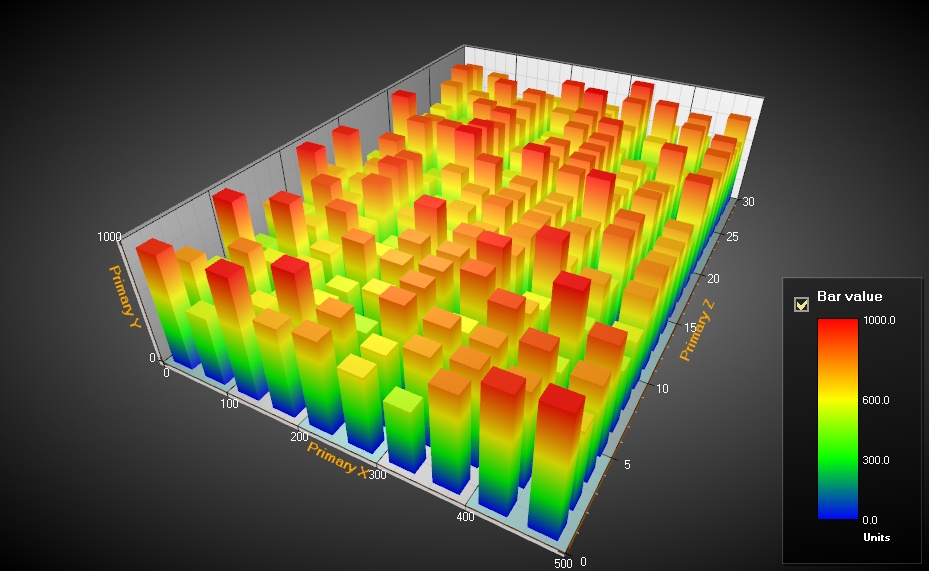
\includegraphics[width=\textwidth,height=\figureheight]{images/introduction/financial}
        \caption{A heat map of financial data. \protect\footnotemark}
        \label{fig:heat_map_financial}
    \end{subfigure}
    \begin{subfigure}[b]{\figurewidth}
        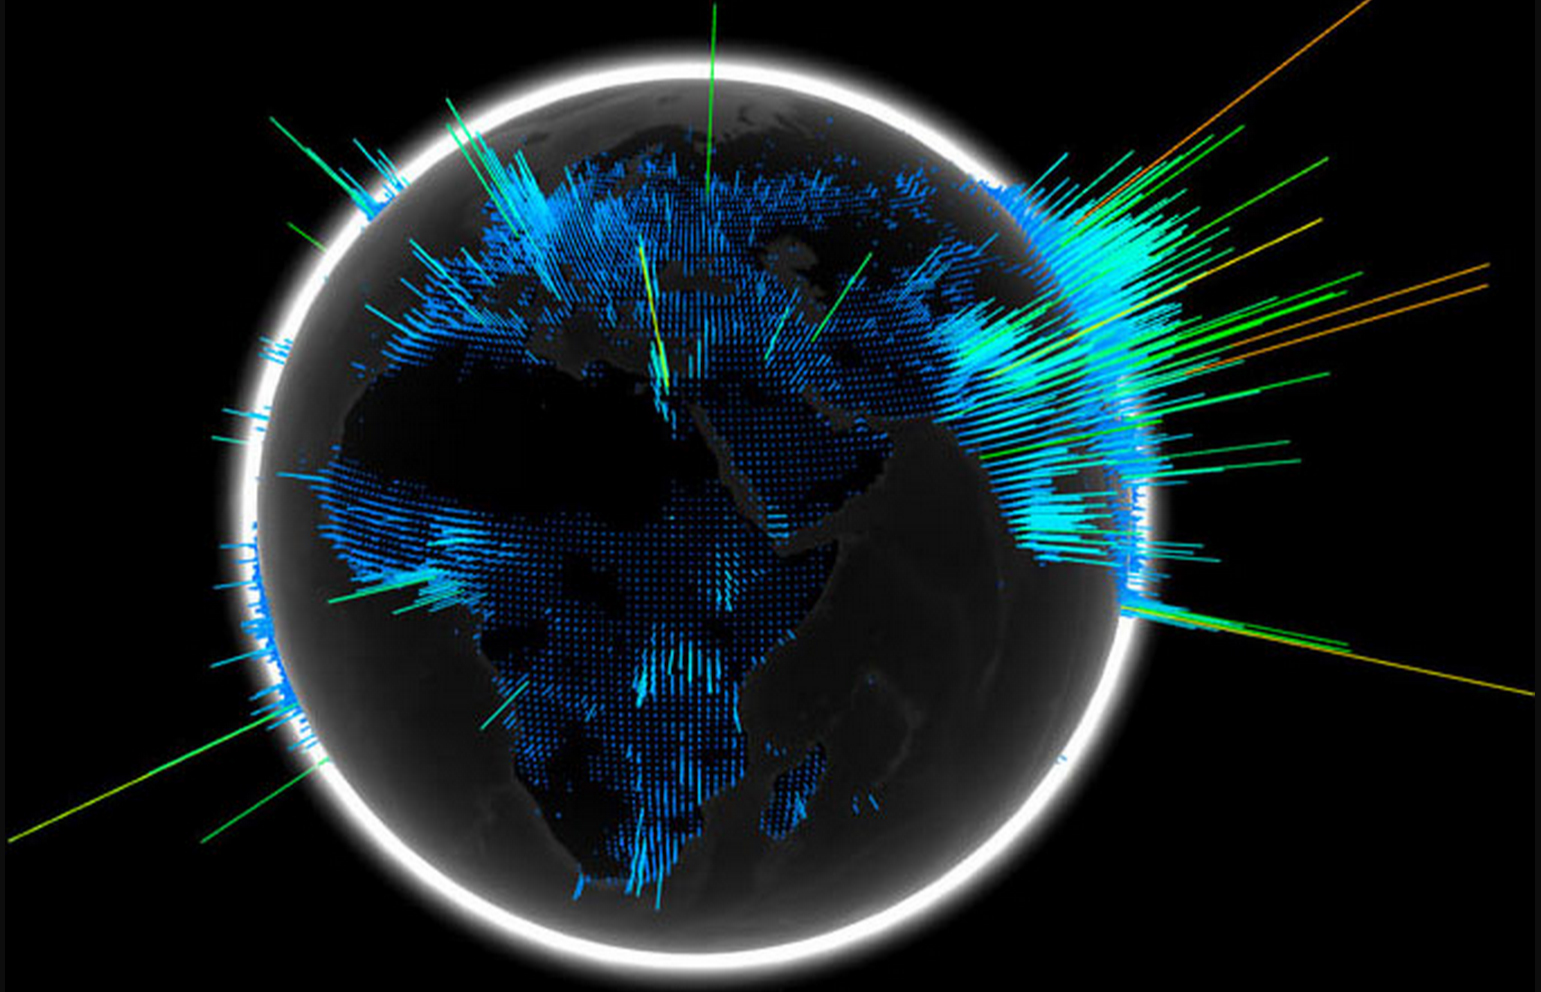
\includegraphics[width=\textwidth,height=\figureheight]{images/introduction/globe}
        \caption{WebGL globe. \protect\footnotemark}
        \label{fig:webgl_globe}
    \end{subfigure}
	\caption[3D representations]{Two different ways of representing 3D data.}
	\label{fig:3d_representations}
\end{figure}

\addtocounter{footnote}{-2}
\stepcounter{footnote}\footnotetext{\bibentry{tuomainen2014financial}}
\stepcounter{footnote}\footnotetext{\bibentry{google2011globe}}


	There is a secondary focus in analysing the performance and scalability between the visualisations, so the system can be designed to cope with large datasets and extended in the future. The primary goals of this project are to:

	\begin{itemize}
		\item Visualise a large dataset in a time efficient manner.
		\item Provide filters to the user and ensure the data can be understood and interpreted without training.
		\item Create visualisations that can be applied to multiple datasets.
		\item Integrate the results into the teaching analytics component of the group project.
		\item Explore how 3D visualisations can effectively convey information.
		\item Apply the visualisations to real datasets and ensure they are scalable.
	\end{itemize}

	The key deliverables of this project have been split into three categories: basic, intermediate and advanced.

	The \emph{basic deliverables} entail developing the implementation for a single visualisation, which should resemble Figure~\ref{fig:heat_map_financial}, with a small, generated dataset. This visualisation will have interactions for panning, zooming and rotating enabling users to navigate the scene.

	The \emph{intermediate deliverables} are concerned with providing users with the ability to filter data, so they are able hide particular information shown on the visualisation. This set of deliverables will also see the implementation of another visualisation, similar to Figure~\ref{fig:webgl_globe}, which will initially be applied to a large, generated dataset. The final stage of these deliverables involves applying real datasets, as outlined in Section~\ref{sec:dataset}, to both visualisations.

	The core \emph{advanced deliverables} requires integrating a third visualisation, based on the two developed in the basic and intermediate deliverables, into the group project for the teaching analytics component. Other deliverables include analysing the scalability and computational power to render the visualisations, performing a user study to measure the usefulness of the visualisations and incorporating multi-touch gestures such as pan, pinch, zoom and rotate.
	
}

\section{Research questions} {
\label{sec:research_questions}

	% Geovisualisations should effectively display geospatial information in order for a user to establish decision-making processes. 

	The usability, scalability between small and large datasets and computer performance must be considered when a geovisualisation is displayed in a web environment. These concerns result in the following research questions, which will be explored throughout this thesis:

	\begin{itemize}
		\item How can a geovisualisation be visualised in WebGL?
		\item How does a geovisualisation perform across small and large datasets?
		\item How can different datasets be applied to 3D geovisualisations?
		\item Do particular colours have any significant effect on the usability of a geovisualisation?
		\item Do particular filters aid in the analysis of a geovisualisation?
	\end{itemize}

}
